\documentclass{article}
\usepackage[utf8]{inputenc}
\usepackage{amssymb}
\usepackage{amsmath}
\usepackage{algorithm}
\usepackage{import}
\usepackage{algcompatible}
\usepackage{algpseudocode}
\usepackage{parskip}
\usepackage{minted}
\usepackage{commath}
\usepackage{tikz}
\usepackage{hyperref}

\usepackage[margin=2.2cm]{geometry}

\title{Theory Assignment-4: ADA Winter-2024}
\author{Rachit Arora (2022384) \and Mahi Mann (2022272)}

\date{}
\begin{document}

\maketitle

\section{Assumptions}

\begin{itemize}
    \item It is assumed that the input graph is a Directed Acyclic Graph, and no detection for incorrect input is required.

    \item By definition, $s$ and $t$ are always \emph{s-t cut} vertices, so they are mentioned as \emph{trivial s-t cut vertices} in the implementation, given a path from $s$ to $t$ exists. 
\end{itemize}

\section{Preprocessing}
% Your preprocessing steps go here

2 empty adjacency lists of sufficiently large size will be required.

\section{Algorithm Description}

\textbf{Note}: The graph is $G = (V,E)$, the start node is $s$ and the target node is $t$.

\begin{enumerate}
    \item First, since we are given a Directed Acyclic Graph, it makes sense to topologically sort the nodes. 

    The toposort will be done using a variant of DFS, where at the end of every DFS call, the node will be pushed to an array, and the array will be reversed later to get a topologically sorted order from left to right. 

    \item We will remove the nodes which were not reachable by node $s$ in the DFS that we perfomed (because every path from $s$ to $t$ starts from $s$, and since no path from $s$ to those nodes exists, they cannot occur on a path from $s$ to $t$ and therefore cannot be \emph{s-t cut vertices}. So, it is safe to remove them from the graph.) 

    (\textbf{Note}: this step removes all nodes before $s$ in the topologically sorted order as well, so we do not need to do that step in post-processing. Proved in the "Proof of Correctness" section.)

    \item Similarly, we remove the nodes such that there is no path from that node to node $t$, since for a node to be an \emph{s-t cut vertex}, at least one path from the node to $t$ has to exist. Thus, we can safely remove them from the graph. 

    (\textbf{Note}: this step removes all nodes after $t$ in the topologically sorted order as well, so we do not need to do that step in post-processing. Proved in the "Proof of Correctness" section.)

    We can do this by performing a DFS on $G^R$ starting from $t$. All nodes not traversed in this DFS will be removed from the graph.

    \textbf{At this point in the algorithm, every node in the graph is reachable from $s$, and every node can reach $t$, and therefore, there is a path going from $s$ to $t$ through every node.}

    \item Now, we will initialise an empty set $S$, which will be our final set of \emph{s-t cut vertices} by the time this algorithm ends. 

    \item Initialise a variable $counter$ to 0. 

    \newpage

    \item We will iterate through every node $q$ in topologically sorted order and do the following:
        \begin{enumerate}
            \item Set $counter$ to $counter - e_i$ where $e_i$ is the number of incoming edges at $q$. 
            \item If $counter$ is 0, add $q$ to $S$.

            \item Set $counter$ to $counter + e_o$, where $e_o$ is the number of edges that initiate from $q$ (i.e. outgoing edges).
        \end{enumerate}

        \textbf{Note:} Suppose there were $n_f$ remaining nodes in the graph after step 3. Then, step 6 has $O(n_f + m)$ constant-time operations where $m$ is the number of edges in the graph.  
    
    \item Remove $s$ and $t$ from $S$.
    \item Return the final answer, $S$, the set of all \emph{s-t cut vertices}, excluding $s$ and $t$.

    The idea of why the $counter$ step works is as follows:

    \begin{itemize}
        \item \textbf{Whenever $counter$ is 0, an equal number of incoming and outgoing edges was discovered. Thus, every possible path going from $s$ can extend to that node.}
        \item \textbf{Whenever $counter$ is greater than 0 after a node iteration, it means that there are paths to $t$ which do not go through that node, and the graph remains connected.  }
        \item $counter$ can never be negative in a topologically sorted order, as we will prove in the "Proof of Correctness" section.
    \end{itemize}

\end{enumerate}

\section{Complexity Analysis}
% Analyze the time and space complexity of your algorithm

\textbf{Note:} We will denote $n$ and the number of nodes in the graph, and $m$ as the number of edges in the graph. 

\subsection*{Step 1}

Step 1 is a topological sort. We can implement this in $O(n + m)$ time because we only need to add a single $O(1)$ operation to the end of every DFS call on $n$ nodes. 

\textbf{This takes $O(m+n)$ time.}

\subsection*{Steps 2 and 3}

These steps remove nodes and edges from the graph. Let $G = (V,E)$ initially. 

We will have an arrays which will mark vertices and edges that are to be removed so that we can access their "status of removal" in $O(1)$ time. 

So, first we will iterate through all the nodes to see which is included. This will take $O(n)$ time. 

Then, we will check all edges, which takes $O(m)$ time.

\textbf{So, in total, creating the new graph takes $O(m + n)$ time.}

\subsection*{Steps 4 and 5}

\textbf{2 $O(1)$ operations, thus $O(1)$ time.}

\subsection*{Step 6}

Incoming edges for each node can be precomputed in step 1. Thus, the "incoming" part of the $counter$ step will take $O(1)$ time for $n$ nodes, therefore $O(n)$ time in total.

Outgoing edges are a little more complicated, because we have to check each edge in a node's adjacecy list manually. This will take $O(m)$ time in total.

\textbf{Therefore, Step 6 takes $O(m+n)$ time.}

\subsection*{Step 7}

$O(n)$ \textbf{time, as we simply need to iterate through all nodes in $S$ and check whether they are $s$ or $t$.}

\subsection*{Step 8}

$O(1)$ time.

\textbf{So in total, since every step is at most $O(m+n)$ time, the algorithm runs in $O(m+n)$ time.}


% \newpage 
% \section{Pseudocode}

% \begin{algorithm}[H]
% \caption{Finding Cut Vertices}
% \begin{algorithmic}[1]
    % \State Initialize arrays $vis1[N]$, $vis2[N]$, and $incident[N]$ with zeros
    % \State Initialize an empty list $toposorted$
    % \Function{DFS1}{$s$}
        % \State $vis1[s] \gets 1$
        % \For{each vertex $v$ in $adj[s]$}
            % \If{$vis1[v] = 0$}
                % \State \Call{DFS1}{$v$}
            % \EndIf
            % \State $incident[v] \gets incident[v] + 1$
        % \EndFor
        % \State Add $s$ to $toposorted$
    % \EndFunction
    % \Function{DFS2}{$t$}
        % \State $vis2[t] \gets 1$
        % \For{each vertex $v$ in $adjrev[t]$}
            % \If{$vis2[v] = 0$}
                % \State \Call{DFS2}{$v$}
            % \EndIf
        % \EndFor
    % \EndFunction
    % \State Initialize arrays $vis1$, $vis2$, and $incident$
    % \State Input $n$, $m$, $s$, and $t$
    % \State Input the edges and construct the graph
    % \State \Call{DFS1}{$s$}
    % \State \Call{DFS2}{$t$}
    % \If{$vis1[t] = 0$}
        % \State Output "No cut vertices"
        % \State \textbf{return}
    % \EndIf
    % \State Reverse $toposorted$
    % \State Initialize $cnt \gets 0$ and an empty list $ans$
    % \For{each vertex $node$ in $toposorted$}
        % \If{$vis2[node] = 0$}
            % \State \textbf{continue}
        % \EndIf
        % \State $cnt \gets cnt - incident[node]$
        % \If{$cnt = 0$}
            % \State Add $node$ to $ans$
        % \EndIf
        % \For{each vertex $edge$ in $adj[node]$}
            % \If{$vis2[edge]$}
                % \State $cnt \gets cnt + 1$
            % \EndIf
        % \EndFor
    % \EndFor
    % \For{each vertex $item$ in $ans$}
        % \State Output $item$
    % \EndFor
% \end{algorithmic}
% \end{algorithm}

\section{Proof of Correctness}
% Provide the proof of correctness for your algorithm

\section*{Addendum 1: C++ implementation}

\inputminted{cpp}{stcut.cpp}

\section*{Addendum 2: Test cases}

\begin{figure}
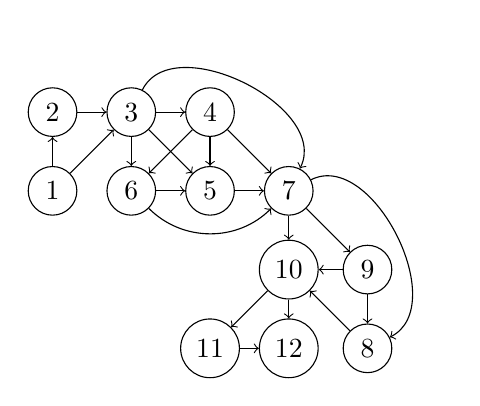
\begin{tikzpicture}[->, nodes={draw, circle}, scale=0.5]

  \node (1) {1};
  \node (2) [above of=1] {2};
  \node (3) [right of=2] {3};
  \node (4) [right of=3] {4};
  \node (6) [below of=3] {6};
  \node (5) [right of=6] {5};
  \node (7) [right of=5] {7};
  \node (10) [below of=7] {10};
  \node (9) [right of=10] {9};
  \node (8) [below of=9] {8};
  \node (12) [left of=8] {12};
  \node (11) [left of=12] {11};

  \path (1) edge (2);
  \path (1) edge (3);
  \path (2) edge (3);
  \path (3) edge (4);
  \path (4) edge (5);
  \path (3) edge (6);
  \path (3) edge (5);
  \path (4) edge (6);
  \path (6) edge (5);
  \path (4) edge (7);
    \path (3) edge [bend left=90](7);
  \path (5) edge (7);
  \path (6) edge [bend right = 45](7);
    \path (7) edge [bend left=90](8);
  \path (7) edge (9);
  \path (7) edge (10);
  \path (9) edge (8);
  \path (9) edge (10);
  \path (8) edge (10);
  \path (10) edge (11);
  \path (10) edge (12);
  \path (11) edge (12);
\end{tikzpicture}
\end{figure}

\begin{figure}
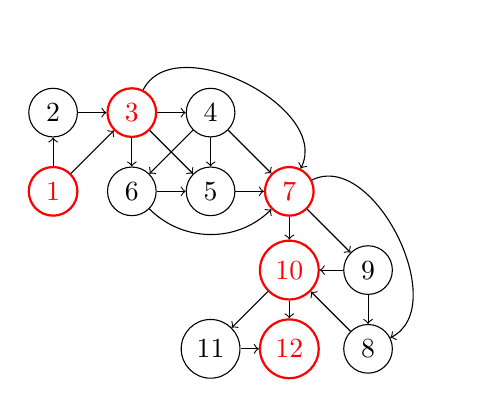
\begin{tikzpicture}[->, nodes={draw, circle}, scale=0.5]

  \node (1) [red, thick]{1};
  \node (2) [above of=1] {2};
  \node (3) [red, thick, right of=2] {3};
  \node (4) [right of=3] {4};
  \node (6) [below of=3] {6};
  \node (5) [right of=6] {5};
  \node (7) [red, thick][right of=5] {7};
  \node (10) [red, thick, below of=7] {10};
  \node (9) [right of=10] {9};
  \node (8) [below of=9] {8};
  \node (12) [red, thick][left of=8] {12};
  \node (11) [left of=12] {11};

  \path (1) edge (2);
  \path (1) edge (3);
  \path (2) edge (3);
  \path (3) edge (4);
  \path (4) edge (5);
  \path (3) edge (6);
  \path (3) edge (5);
  \path (4) edge (6);
  \path (6) edge (5);
  \path (4) edge (7);
    \path (3) edge [bend left=90](7);
  \path (5) edge (7);
  \path (6) edge [bend right = 45](7);
    \path (7) edge [bend left=90](8);
  \path (7) edge (9);
  \path (7) edge (10);
  \path (9) edge (8);
  \path (9) edge (10);
  \path (8) edge (10);
  \path (10) edge (11);
  \path (10) edge (12);
  \path (11) edge (12);

\end{tikzpicture}
\end{figure}



\section*{Addendum 3: People discussed with}

Swapnil Panigrahi, Rohak Kansal and Sahil Gupta.


\vspace*{\fill}
\begin{center}
    $\square \square \square \square$
    \\
    thank you.
\end{center}
\vspace*{\fill}

\end{document}
